\documentclass{beamer}

\input{../../spec_files/course_preamble.tex}
\subtitle{Foundations of Neuro-Symbolic AI}
\date{Summer Term 2026}
\author[FONS]{Alex Goessmann}
\institute[]{
    University of Applied Science Würzburg-Schweinfurt (THWS)
%    Weierstrass Institute for Applied Analysis and Stochastic
}

\newcommand{\setslidetitledate}[2]{
    \title[#1]{
        \coursechapterone \\
        {\huge #1}
    }
    \date{#2}
}

\newcommand{\stantikzpic}[1]{
    \begin{center}
    \begin{tikzpicture}[scale=0.35, thick]
    #1
    \end{tikzpicture}
    \end{center}
}

%\newcommand{\techwstitle}{
%\small
%%Workshop \\
%Logik für Erklärbare KI:
%Technische Einführung in das ENEXA Projekt}
%\newcommand{\smalltechwstitle}{ENEXA Workshop}

%\newcommand{\techwsdate}{15.+16. July, 2024}

%\newcommand{\techwsauthors}{
%Alex Goessmann
%}

%\newcommand{\techwsinclude}{
%	\usepackage{../../spec/beamercolorthemeclaw}
%	\usepackage{/Users/alexgoessmann/Documents/ENEXA/latex_macros/beamer_template/beamerfontthemeclaw}
%	\usepackage{/Users/alexgoessmann/Documents/ENEXA/latex_macros/beamer_template/beamerinnerthemeclaw}
%	\usepackage{/Users/alexgoessmann/Documents/ENEXA/latex_macros/beamer_template/beamerouterthemeclaw}
%
%	\input{/Users/alexgoessmann/Documents/ENEXA/latex_macros/packages.tex}
%	\input{/Users/alexgoessmann/Documents/ENEXA/latex_macros/macros.tex}
%	\input{/Users/alexgoessmann/Documents/ENEXA/latex_macros/macros_tc.tex}
%	\input{/Users/alexgoessmann/Documents/ENEXA/latex_macros/tikz_blocks.tex}
%
%	\subtitle{\techwstitle}
%	\date[\techwsdate]{\techwsdate}
%	\author[\smalltechwstitle]{\techwsauthors}
%	\institute[]{\eupic}
%}

\newcommand{\coursechapterone}{I-Logical Approaches}
\newcommand{\coursechaptertwo}{II-Probabilistic Approaches}
\newcommand{\coursecahterthree}{III-Statistical Models of Knowledge Graphs}
\newcommand{\coursechapterfour}{IV-Quantum Machine Learning}

\newcommand{\techwschapterone}{I-Tensors}
\newcommand{\techwschaptertwo}{II-Probabilities}
\newcommand{\techwschapterthree}{III-Logics}
\newcommand{\coursechapterthree}{IV-Applications}

\newcommand{\eupic}{
    \begin{center}
    %
\includegraphics[width=4cm]{/Users/alexgoessmann/Documents/ENEXA/latex_macros/images/fundedEU.png}
    \end{center}
}

%\newcommand{\enexadateveublock}{
%    \begin{center}\begin{tikzpicture}
%    %\node [anchor=center] at (0,0) {\includegraphics[width = 1.5cm]{/Users/alexgoessmann/Documents/ENEXA/latex_macros/images/DATEV.png}};
%    %\node [anchor=center] at (2.5,0.5) {
\includegraphics[width = 3.5cm]{/Users/alexgoessmann/Documents/ENEXA/latex_macros/images/enexa.png}};
%    %\node [anchor=center] at (2.55,-0.5) {
\includegraphics[width = 3cm]{/Users/alexgoessmann/Documents/ENEXA/latex_macros/images/fundedEU.png}};
%    \end{tikzpicture}\end{center}
%}


%% OLD
\newcommand{\aselectionvariable}{L}
\newcommand{\vselectionvariable}{L}
\newcommand{\fselectionvariable}{L}
\newcommand{\cselectionvariable}{L}
\newcommand{\individualorder}{n}
\newcommand{\variableof}[1]{\indvariableof{#1}}
\newcommand{\sindex}{s}
\newcommand{\pindex}{p}
\newcommand{\oindex}{o}
\newcommand{\exquery}{q}
%\newcommand{\datapointof}[1]{x^{#1}}
\newcommand{\atomicqueryof}[1]{g_{#1}}
\newcommand{\facsystem}{\shortcatvariables}
\newcommand{\margprobof}[1]{\probat{#1}}
\newcommand{\mlnprobabilityof}[1]{\expdistof{#1}}
%\newcommand{\oldenexadateveublock}{
%	\begin{center}
%	\begin{minipage}{0.2\textwidth}
%		\begin{center}
%			\includegraphics[width = 2.5cm]{images/DATEV.png}
%		\end{center}
%	\end{minipage}
%	\begin{minipage}{0.55\textwidth}
%		\begin{center}
%			
\includegraphics[width=5.5cm]{images/enexa.png} \\
%			
\includegraphics[width=5.5cm]{images/fundedEU.png} \\
%		\end{center}
%	\end{minipage}
%	\end{center}
%}

\newcommand{\showoutlineatsection}{
    \AtBeginSection[ ]
    {
        \begin{frame}{Outline}
        \tableofcontents[currentsection]
        \end{frame}
    }
    %\begin{frame}{Outline}
    %\tableofcontents
    %\end{frame}

    \addtocounter{framenumber}{-1}
}

\tikzset{
    midarrow/.style={
        postaction={decorate},
        decoration={
            markings,
            mark=at position 0.5 with {\arrow{Straight Barb[length=4pt, width=5pt]}}
            % Or use {Stealth}, {To}, or {Latex[open]}
        }
    },
    midbackarrow/.style={
        postaction={decorate},
        decoration={
            markings,
            mark=at position 0.5 with {\arrow{<[Straight Barb[length=4pt, width=5pt]]}}
        }
    },
    >>-/.style={midarrow},
    <<-/.style={midbackarrow}
}

\newcommand{\drawtnreasonarchitecture}{
    \draw[dashed] (-30,15) -- (12,15) -- (12,-3) -- (-30,-3) -- (-30,15);

    \draw[] (-10,10) rectangle (10,14);
    \node [anchor=center] at (0,12) {\corelabelsize \spapplication{}};

    \node [anchor=west] at (-29,12) {\layerthreespec};
    \draw[dashed] (-30,9) -- (12,9);
    \node [anchor=west] at (-29,6) {\layertwospec};

    \draw[->] (6,10) -- (6,8);
    \draw[] (2,4) rectangle (10,8);
    \node [anchor=center] at (6,6) {\spreasoning{}};
    \draw[->] (6,4) -- (6,2);

    \draw[->] (-5,10) -- (-5,8);
    \draw[] (-10,4) rectangle (0,8);
    \node [anchor=center] at (-5,6) {\sprepresentation{}};
    \draw[->] (-5,4) -- (-5,2);

    \draw[dashed] (-30,3) -- (12,3);
    \node [anchor=west] at (-29,0) {\layeronespec};

    \draw[] (-10,-2) rectangle (10,2);
    \node [anchor=center] at (0,0) {\spengine};
}

\setslidetitledate{
    Constraint Satisfaction Problems
}{
    April 27, 2026
}

\begin{document}

    {\frame[plain]{\titlepage}}

    \showoutlineatsection


    \section{Examples}

    \begin{frame}{Graph Coloring}

        \begin{block}{Graph Coloring Problem}
            Given a graph $\graph=(\nodes,\edges)$ and $\catdim$ colors, find a coloring of the nodes, such that adjacent nodes have different colors.
        \end{block}

            {\bf Example:} Paint the states of australia\\
        \begin{minipage}{0.45\textwidth}
            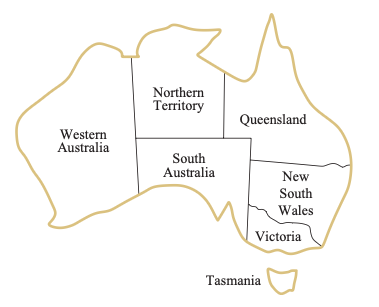
\includegraphics[width=5cm]{img/russel_australia}
        \end{minipage}
        \begin{minipage}{0.45\textwidth}
            \begin{itemize}
                \item How many colors are required?
                \item How many possible colorings can be done?
            \end{itemize}
        \end{minipage}
    \end{frame}

    \begin{frame}{Representation of Graph Coloring}
        We model the problem:
        \begin{itemize}
            \item Enumerate the colors by the state set $[\catdim]=\{0,\ldots,\catdim-1\}$
            \item For each node $\node\in\nodes$ we define a variable $\catvariableof{\node}$
        \end{itemize}
        To each edge $\edge=\{\node_{0},\node_{1}\}$ the "different" constraint matrix
        \begin{align*}
            \hypercoreofat{\mathrm{diff},\{\node_0,\node_1\}}{\catvariableof{\node_{0}},\catvariableof{\node_{1}}}
            = \onesat{\catvariableof{\node_{0}},\catvariableof{\node_{1}}} - \identityat{\catvariableof{\node_{0}},\catvariableof{\node_{1}}} \, .
        \end{align*}
        with off-diagonal support enforces different color constraint.
        \begin{align*}
            \hypercoreofat{\{\nodeof{0},\nodeof{1}\}}{\catvariableof{\nodeof{0}},\catvariableof{\nodeof{1}}}
            =\coloredmatrixof{
                0 & 1 & \cdots & 1  \\
                1 & \ddots & \ddots & \vdots \\
                \vdots & \ddots & \ddots & 1 \\
                1 & \cdots & 1 & 0
            }{\catvariableof{\nodeof{0}},\catvariableof{\nodeof{1}}}
        \end{align*}
    \end{frame}

    \begin{frame}{Example: Painting states of australia}
        Let us paint the states of australia with $3$ colors:
        \begin{itemize}
            \item $7$ color variables $\catvariableof{\cdot}$ of leg dimension $\catdim=3$
            \item $9$ edges between neighbored states $\nodeof{0}$ and $\nodeof{1}$, which are decorated by the $3x3$ constraint matrix
        \end{itemize}
        \begin{minipage}{0.54\textwidth}
            \begin{align*}
                &\hypercoreofat{\{\nodeof{0},\nodeof{1}\}}{\catvariableof{\nodeof{0}},\catvariableof{\nodeof{1}}} \\
                &\quad=
                \coloredmatrixof{
                    0 & 1 & 1 \\
                    1 & 0 & 1 \\
                    1 & 1 & 0
                }{\catvariableof{\nodeof{0}},\catvariableof{\nodeof{1}}}
            \end{align*}
        \end{minipage}
        \begin{minipage}{0.45\textwidth}
            \stantikzpic{

    \drawvariablenode{0}{0}{$\catvariableof{WA}$}{WA}
    \drawvariablenode{5}{3}{$\catvariableof{NT}$}{NT}
    \drawvariablenode{5}{-2}{$\catvariableof{SA}$}{SA}
    \drawvariablenode{10}{3}{$\catvariableof{Q}$}{Q}
    \drawvariablenode{10}{-2}{$\catvariableof{NSW}$}{NSW}
    \drawvariablenode{7.5}{-6}{$\catvariableof{V}$}{V}

    \drawvariablenode{12.5}{-5}{$\catvariableof{T}$}{T}

    \draw (WA) -- (NT);
    \draw (WA) -- (SA);
    \draw (NT) -- (SA);
    \draw (NT) -- (Q);
    \draw (SA) -- (Q);
    \draw (SA) -- (V);
    \draw (SA) -- (NSW);
    \draw (Q) -- (NSW);
    \draw (NSW) -- (V);
}
        \end{minipage}
    \end{frame}



    %\section{Sudoku}

    \begin{frame}{Representation of Sudoku}

        By hidden variables storing digit at a field, digit positions in rows, columns and squares.

        Computation perspective: Hidden variables computing the atomic variables.
        Speciality of Sudoku constraint: Can disentangle to basis vector $\fbasis$ when position variable

    \end{frame}

    \begin{frame}{Adjusting possible variable assignments}

        Easiest inference scheme: Adjusting possible variable assignments

    \end{frame}



    \section{Generalized unit propagation}

    \begin{frame}{Disentangling the constraint network}

        Example for graph coloring: When a color is known, the corresponding edges can be dropped.

        Goal of inference: Disentangling the constraint network
        \begin{itemize}
            \item Satisfiability when all local vectors non-vanishing
            \item Read off the solutions as a cartesian product of local conditions
        \end{itemize}

    \end{frame}


    \begin{frame}{Generalized unit propagation}

        Comparison with unit propagation so far:
        \begin{itemize}
            \item Works with arbitrary constraints (shape, values), while so far on unit clauses
            \item
        \end{itemize}

        Known as AC-3: Enforcing arc-consistency.

    \end{frame}

    \begin{frame}{Generalized unit propagation algorithm}

        \begin{algorithm}[H]
            \begin{algorithmic}
                \Require Constraint network $\extnet$
                \Ensure Equivalent constraint network $\extnet$, with potentially less connectivity in $\graph$
                \iosepline
                \State Initialize a queue $Q$ of unary edges in $\graph$
                \While{$Q$ not empty}
                    \State $\{\node\}=Q.pop()$
                    \For{$\edge\in\edges\wcols \node\in\edge$}
                        \State $\hypercoreofat{\edge}{\catvariableof{\edge}}
                        \algdefsymbol \contractionof{\hypercoreofat{\edge}{\catvariableof{\edge}},\hypercoreofat{\{\node\}}{\catvariableof{\node}}}{\catvariableof{\edge}}$
                    \State Try to split $\hypercoreofat{\edge}{\catvariableof{\edge}}$ into a vector $\node$ and a tensor $\edge\backslash\{\node\}$
                    \If{Split successful and $\cardof{\edge\backslash\{\node\}}=1$}
                        \State $Q.push(\edge\backslash\{\node\})$
                    \EndIf
                    \EndFor
                \EndWhile
                \State \Return $\extnet$
            \end{algorithmic}
        \end{algorithm}

    \end{frame}


    %\section{Solution by forward chaining}

%    \begin{frame}{Solution by forward chaining like method}
%
%        Here: AC-3 a generalization of forward chaining to leg dimensions $\catdim>2$!
%
%        Can show:
%        AC-3 and forward chaining do the most basic inference scheme, i.e. keeping track of possible assignments based on single constraint matrices.
%
%    \end{frame}
%
%    \begin{frame}{Arc consistency}
%
%        More generic inference rules: Generating locally consistent assignments.
%    \end{frame}

%    \begin{frame}{Edge inference scheme}
%
%        Each node color gets assigned a vector of possibilities.
%        \begin{align*}
%            \vectorofat{\node_0}{\catvariableof{\node_0}}
%            = \nonzeroof{
%                \contractionof{
%                    \vectorofat{\node_0}{\catvariableof{\node_0}},
%                    \hypercoreofat{\edge}{\catvariableof{\node_{0}},\catvariableof{\node_{1}}},
%                    \vectorofat{\node_0}{\catvariableof{\node_1}}
%                }{\catvariableof{\node_0}}
%            }
%        \end{align*}
%
%    \end{frame}


    \section{Backtracking search}

    \begin{frame}{Contraction properties of the "different" constraint}

        If one node is known (i.e. encoded as a basis vector), then constraint disentangles.
        (This holds for any constraint!)

        If multiple possibilities, then entanglement remains.

        Unit propagation helps only, when the color of one node $\nodeof{0}$ is known:
        \begin{align*}
            &\nzcontractionof{
                \vectorat{\catvariableof{\nodeof{0}}},
                \hypercoreofat{\{\nodeof{0},\nodeof{1}\}}{\catvariableof{\nodeof{0}},\catvariableof{\nodeof{1}}}
            }{\catvariableof{\nodeof{1}}} \\
            & \quad =
            \begin{cases}
                \onesat{\catvariableof{\nodeof{1}}} - \onehotmapofat{\headindex}{\catvariableof{\nodeof{1}}} & \text{if $\vectorat{\catvariableof{\nodeof{0}}}$ only at $\headindex$ supported} \\
                \onesat{\catvariableof{\nodeof{1}}} & \text{else}
            \end{cases}
            %% WRONG!
%            \underbrace{\onesat{\catvariableof{\nodeof{1}}}}_{\text{everywhere supported}}
%            -
%            \underbrace{
%%                \contractionof{
%%                \identityat{\catvariableof{\nodeof{0}},\catvariableof{\nodeof{1}}},
%%                \nonzeroof{\vectorat{\catvariableof{\nodeof{0}}}}
%%                }{\catvariableof{\nodeof{1}}}
%            }_{\text{except for the support of $\vectorat{\catvariableof{\nodeof{0}}}$}}
        \end{align*}

        \begin{block}{Inference by matrix-vector contractions}
            Known colors are communicated along edges.
        \end{block}

        \begin{center}
            \bf But where to find the basis vectors necessary for disentangling the color constraints?
        \end{center}
    \end{frame}



    \begin{frame}{Idea of backtracking}


        Guess an assignment to disentangle a node.
        When running into an inconsistency, guess an alternative assignment.


    \end{frame}

    \begin{frame}{Combination with constraint simplification}

        Do generic unit propagation in an inner loop to simplify constraints before guessing.


    \end{frame}

    \begin{frame}{Example: Painting australias states}

        Take three colors: red, blue, green

        \stantikzpic{
    \only<1>{
        \drawvariablenode{0}{0}{$\catvariableof{WA}$}{WA}
    }
    \only<2->{
        \begin{scope}[red]
            \drawvariablenode{0}{0}{$\catvariableof{WA}$}{WA}
        \end{scope}
    }

    \only<1-3>{
        \drawvariablenode{5}{3}{$\catvariableof{NT}$}{NT}
    }
    \only<3>{
        \fill[green!70!black] (5.5,4.75) circle (0.3cm);
        \fill[blue] (4.5,4.75) circle (0.3cm);
    }
    \only<4->{
        \begin{scope}[green!70!black]
            \drawvariablenode{5}{3}{$\catvariableof{NT}$}{NT}
        \end{scope}
    }

    \only<1-4>{
        \drawvariablenode{5}{-2}{$\catvariableof{SA}$}{SA}
    }
    \only<3>{
        \fill[green!70!black] (5,-3.75) circle (0.3cm);
        \fill[blue] (4,-3.5) circle (0.3cm);
    }
    \only<4>{
        \fill[blue] (4,-3.5) circle (0.3cm);
    }
    \only<5->{
        \begin{scope}[blue]
            \drawvariablenode{5}{-2}{$\catvariableof{SA}$}{SA}
        \end{scope}
    }

    \only<1-6>{
        \drawvariablenode{10}{3}{$\catvariableof{Q}$}{Q}
    }
    \only<4>{
        \fill[red] (10.5,4.75) circle (0.3cm);
        \fill[blue] (9.5,4.75) circle (0.3cm);
    }
    \only<5>{
        \fill[red] (10,4.75) circle (0.3cm);
    }
    \only<6->{
        \begin{scope}[red]
            \drawvariablenode{10}{3}{$\catvariableof{Q}$}{Q}
        \end{scope}
    }

    \only<1-5>{
        \drawvariablenode{10}{-2}{$\catvariableof{NSW}$}{NSW}
        \drawvariablenode{7.5}{-6}{$\catvariableof{V}$}{V}
    }
    \only<6->{
        \begin{scope}[green!70!black]
            \drawvariablenode{10}{-2}{$\catvariableof{NSW}$}{NSW}
        \end{scope}
    }
    \only<6->{
        \begin{scope}[red]
            \drawvariablenode{7.5}{-6}{$\catvariableof{V}$}{V}
        \end{scope}
    }

    \only<1-6>{
        \drawvariablenode{12.5}{-5}{$\catvariableof{T}$}{T}
    }
    \only<7>{
        \begin{scope}[blue]
            \drawvariablenode{12.5}{-5}{$\catvariableof{T}$}{T}
        \end{scope}
    }

    \draw (WA) -- (NT);
    \draw (WA) -- (SA);
    \draw (NT) -- (SA);
    \draw (NT) -- (Q);
    \draw (SA) -- (Q);
    \draw (SA) -- (V);
    \draw (SA) -- (NSW);
    \draw (Q) -- (NSW);
    \draw (NSW) -- (V);
}
        \begin{itemize}
            \item \only<2->{
                Guess $\catvariableof{WA}$ to be red.
            }
            \item \only<3->{
                Consequences for $\catvariableof{NT}$ and $\catvariableof{SA}$: red or green
            }
            \item \only<4->{
                Guess $\catvariableof{NT}$ to be green.
            }
            \item \only<5->{
                As a consequence, $\catvariableof{SA}$ has to be blue.
            }
            \item \only<6->{
                The colors $\catvariableof{Q}$, $\catvariableof{NSW}$, $\catvariableof{V}$ also follow.
            }
            \item \only<7>{
                The variable $\catvariableof{T}$ is disconnected and can be chosen arbitrarly.
            }
        \end{itemize}


    \end{frame}



    \section{Generic inference algorithms}

    \begin{frame}{So far}

        Generalized unit propagation choices subsets $\secgraph$ as:
        \begin{itemize}
            \item Two constraint tensors
            \item One constraint tensor is of order $1$ (i.e. a vector)
        \end{itemize}

        More complex reasoning steps: Contraction of multiple constraint tensors with larger order, keeping only a subset open.

    \end{frame}

    \begin{frame}{Recall: Support tensors}

        Support tensor to a tensor $\hypercorewith$: $\nonzeroof{\hypercorewith}$ with coordinates
        \begin{align*}
            \nonzeroof{\hypercoreat{\indexedshortcatvariables}}
            = \begin{cases}
                  1 & \ifspace \hypercoreat{\indexedcatvariables}\neq 0 \\
                  0 & \text{else}
            \end{cases}
        \end{align*}

        \begin{block}{Invariance under adding support tensor to sub-contractions}
            Any support tensor of a sub-contraction can be added to a tensor network: When $\secgraph$ a sub-hypergraph of $\graph$, then
            \begin{align*}
                \contractionof{\extnetwith}{\nodevariables}
                = \contractionof{\extnetwith,
                    \nonzeroof{\contractionof{\tnetofat{\secgraph}{\nodevariables}}{\catvariableof{\secnodes}}}
                }{\nodevariables}
            \end{align*}
        \end{block}

        In propositional logics, this means:
        \begin{align*}
            \nonzeroof{\contractionof{\extnetwith}{\nodevariables}}
            \models \nonzeroof{\contractionof{\tnetofat{\secgraph}{\nodevariables}}{\catvariableof{\secnodes}}}
        \end{align*}

    \end{frame}




    \begin{frame}{Outlook}

        Sub-contractions model inference rules
        \begin{itemize}
            \item Logics: Modus ponens, resolutions
            \item CSPs: arc-consistency
        \end{itemize}

        Tradeoff in the sub-contraction size:
        \begin{itemize}
            \item Efficiency: Number of possible sub-contractions, computational demand to perform a sub-contraction
            \item Generality: Larger contractions can perform more complex reasoning steps
        \end{itemize}
%
%        Scheduling is a central challenge for efficient inference.
%        Examples:
%        \begin{itemize}
%            \item Forward Chaining
%            \item SLD Resolution
%        \end{itemize}


    \end{frame}


\end{document}













